\subsection{KNeighbors Regressor}

La KNeighbors Regression es un algoritmo de aprendizaje automático que utiliza el concepto de vecinos más cercanos para hacer predicciones. Para determinar cuáles son los vecinos más cercanos, se utiliza una medida de distancia, como la distancia Euclidiana o la distancia de Manhattan.
\newline

El estudio de este modelo ha empezado buscando el número óptimo de vecinos, en nuestro caso se ha entrenado el modelo y ejecutado la validación cruzada para un rango finito de valores desde el 2 hasta el 800. La evolucion de los errores se puede ver en la Figura \ref{Modelos-Lineales-kneigh-Evolucion-score}. Si nos fijamos en la grafica, podemos ver que segun la validación cruzada el número óptimo de vecinos es $28$, un valor que si nos fijamos en su $R^2$ se encuentra de entre los mejores de todo el rango finito de valores.

\begin{figure}[H]
    \centering
    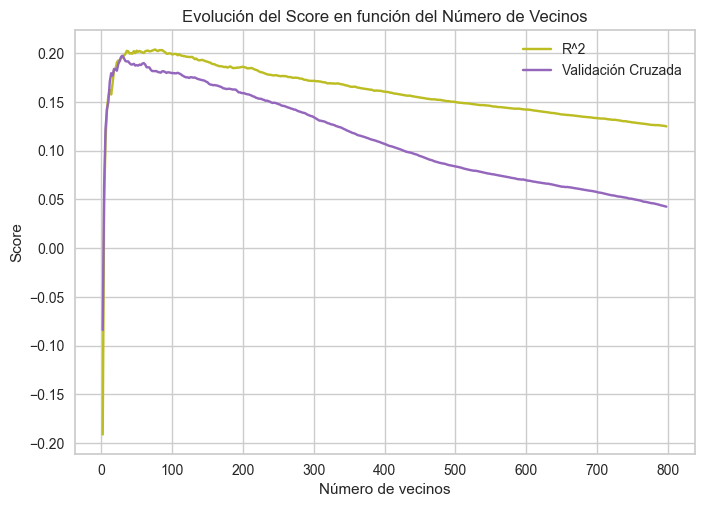
\includegraphics[width=\figsize]{images/linearModelKNeighEvolucionError.png}
    \caption{KNeighbors Regressor: Evolucion del score}
    \label{Modelos-Lineales-kneigh-Evolucion-score}
\end{figure}

De la misma manera que con el resto de modelos testeados, se ha creido oportuno comprovar el tiempo medio de entrenamiento que ha requerido cada modelo, ya que para este proyecto puede parecer una metrica poco significativa, pero para proyectos con conjuntos de datos más grandes puede significar un cambio radical en la estrategia a abrodar. En este modelo se ha obtenido, de media, $0.004$ segundos.

\begin{figure}[H]
    \centering
    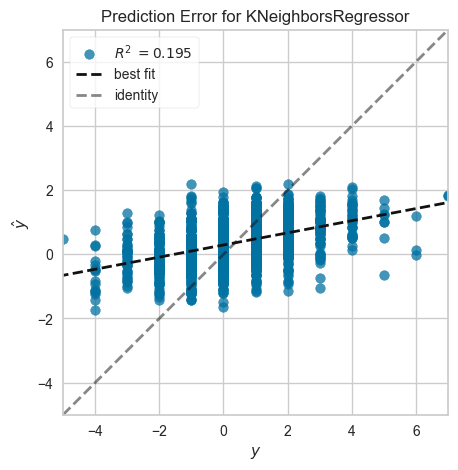
\includegraphics[width=\smallSize]{images/linearModelkNeigh.png}
    \caption{KNeighbors Regressor: Prediccion}
    \label{Modelos-Lineales-kneigh-Evolucion-error}
\end{figure}

Como se ha podido comprovar en la Figura \ref{Modelos-Lineales-kneigh-Evolucion-error} los resultados no son altamente satisfactorios, ya que estamos obteniendo un valor de $R^2$ de $0.195$ y un valor de validación cruzada de $0.196$. Si queremos fijarnos en los valores individuales de la validación cruzada nos podemos fijar en el Cuadro \ref{Modelos-Lineales-kneigh-Validacion-Cruzada}.

\begin{table}[h]
    \centering
    \begin{tabular}{lccccc}
        \textbf{Pliegue} & 1 & 2 & 3 & 4 & 5 \\
        \textbf{Resultado} & 0.23137501 & 0.13387569 & 0.21036481 & 0.14652612 & 0.25953019
    \end{tabular}
    \caption{KNeighbors Regressor: Resultados Validación Cruzada}
    \label{Modelos-Lineales-kneigh-Validacion-Cruzada}
\end{table}